\documentclass{beamer}

\usetheme{Warsaw}
\usepackage{hyperref}
\usepackage{graphicx}
\usepackage{geometry}


\title{PID neural networks for time-delay systems}

\author{Mingkun Yang \\
\texttt{minyan09@student.hh.se}}

\institute{
Halmstad University\\
}
\date{}

\AtBeginSection[]
{
\begin{frame}<beamer>{Outline}
	\tableofcontents[currentsection]
\end{frame}
}

\begin{document}

% \begin{frame}
	% \titlepage
% \end{frame}

% \begin{frame}{Outline}
	% \tableofcontents[pausesections]
% \end{frame}

% \section{Introduction}
% \begin{frame}{PID controller}
	% \begin{itemize}
		% \item
			% not suitable for long time-delay system
		% \item
			% PID parameters are difficult to choose
	% \end{itemize}
% \end{frame}
% \begin{frame}{Artificial neural networks}
	% \begin{itemize}
		% \item
			% slow learning speed
		% \item
			% long weight convergence
		% \item
			% uncertain property
	% \end{itemize}
% \end{frame}
% \begin{frame}{PIDNN}
	% \begin{itemize}
		% \item
			% proportional(P), integral(I) and derivative(D) neurons
		% \item
			% back-propagation
	% \end{itemize}
% \end{frame}

% \section{Structure of PIDNN}
% \begin{frame}{schema}
	% 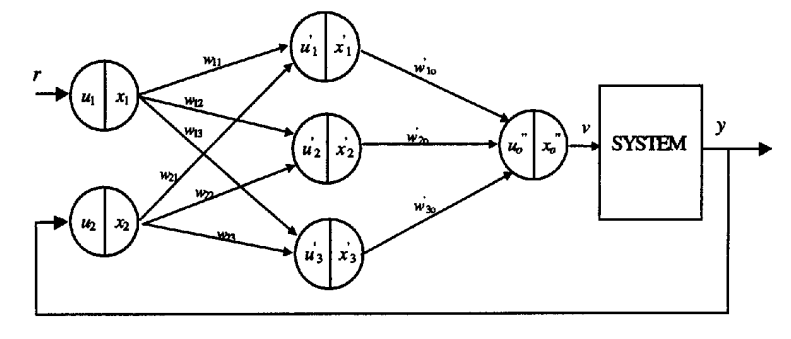
\includegraphics[width=120mm, height=60mm]{structure_pidnn.png}
% \end{frame}

% \section{Algorithm of PIDNN}
% \begin{frame}{Input-output function}
	% $$ x_i(k) = u_i(k) $$
	% $$ x_1^\prime(k) = u_1^\prime(k) $$
	% $$ x_2^\prime(k) = x_2^\prime(k-1) + u_2^\prime(k) $$
	% $$ x_3^\prime(k) = u_3^\prime(k) - u_3^\prime(k-1) $$
	% $$ x_1''(k) = u_1''(k) $$
% \end{frame}
% \begin{frame}{Objective function}
	% $$ J = \sum_{k=1}^n[r(k) - y(k)]^2 $$
	% $$ w_{j0}^\prime(n_0+1) = w_{j0}^\prime(n_0) - \eta_j*\frac{\partial J}{\partial w_{j0}^\prime} $$
	% $$ w_{ij}(n_0+1) = w_{ij}(n_0) - \eta_i*\frac{\partial J}{\partial w_{ij}} $$
% \end{frame}
% \begin{frame}{schema}
	% 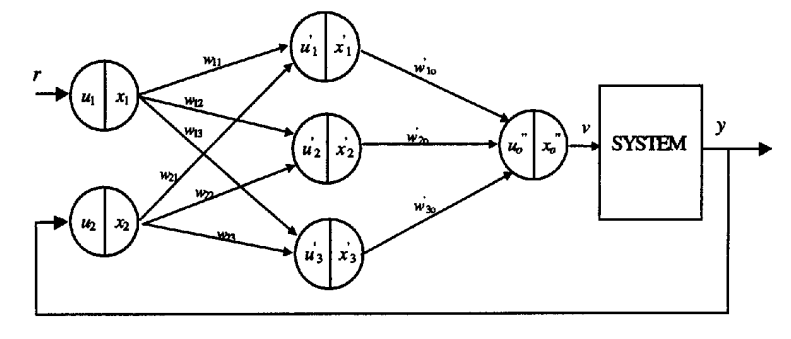
\includegraphics[width=120mm, height=60mm]{structure_pidnn.png}
% \end{frame}

% \section{Result \& Conclusion}
% \begin{frame}{Example}
	% \begin{eqnarray*}
	% y(k+1) &=& 1.368*y(k) - 0.368*y(k-1) \\
		% && + 0.0092*v(k-10) + 0.066*v(k-11)
	% \end{eqnarray*}
% \end{frame}
% \begin{frame}{Using PIDNN}
	% 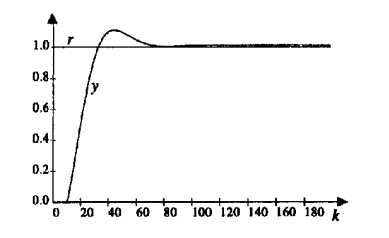
\includegraphics[width=120mm, height=60mm]{pidnn.png}
% \end{frame}
% \begin{frame}{Using PID}
	% 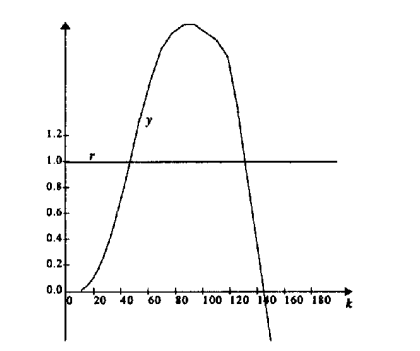
\includegraphics[width=120mm, height=60mm]{pid.png}
% \end{frame}
% \begin{frame}{Conclusion}
	% \begin{itemize}
		% \item
			% No need to calculate the system parameters
		% \item
			% Short convergence time.
	% \end{itemize}
% \end{frame}
\end{document}
